\begin{markdown}
# Этап 4

## Скриншоты
\end{markdown}

\begin{figure}[H]
  \centering
  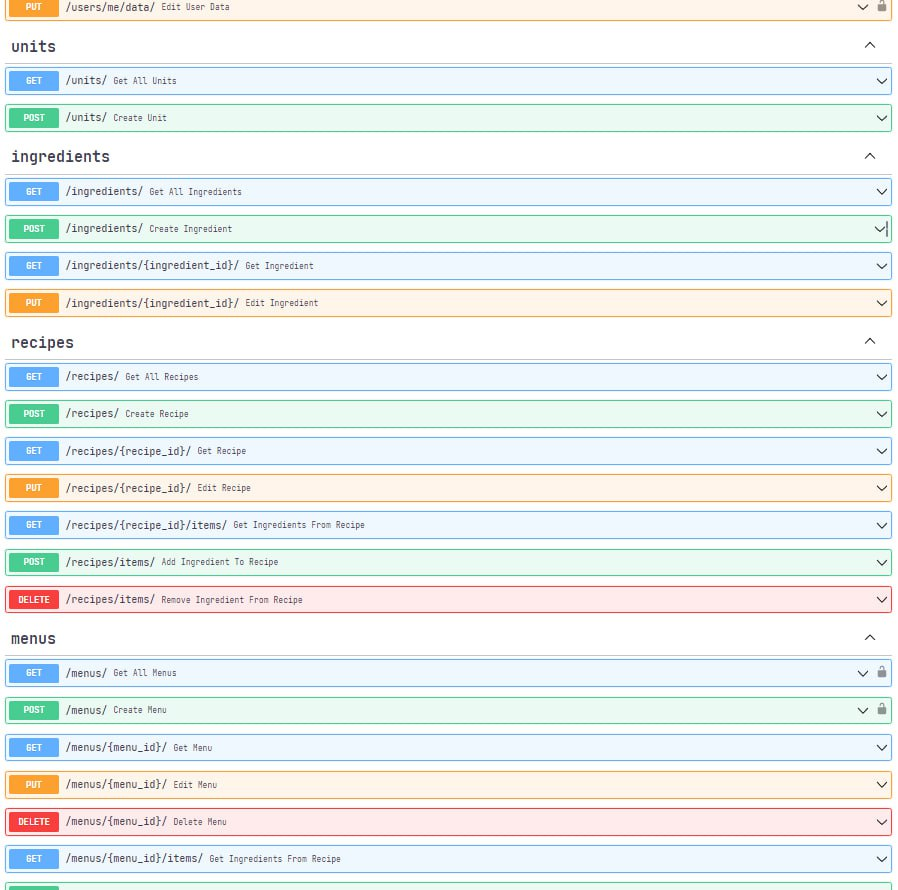
\includegraphics[width=0.9\textwidth]{fig/swagger.jpg}
  \caption{Вырезка из описания Backend API}
\end{figure}

\begin{figure}[H]
  \centering
  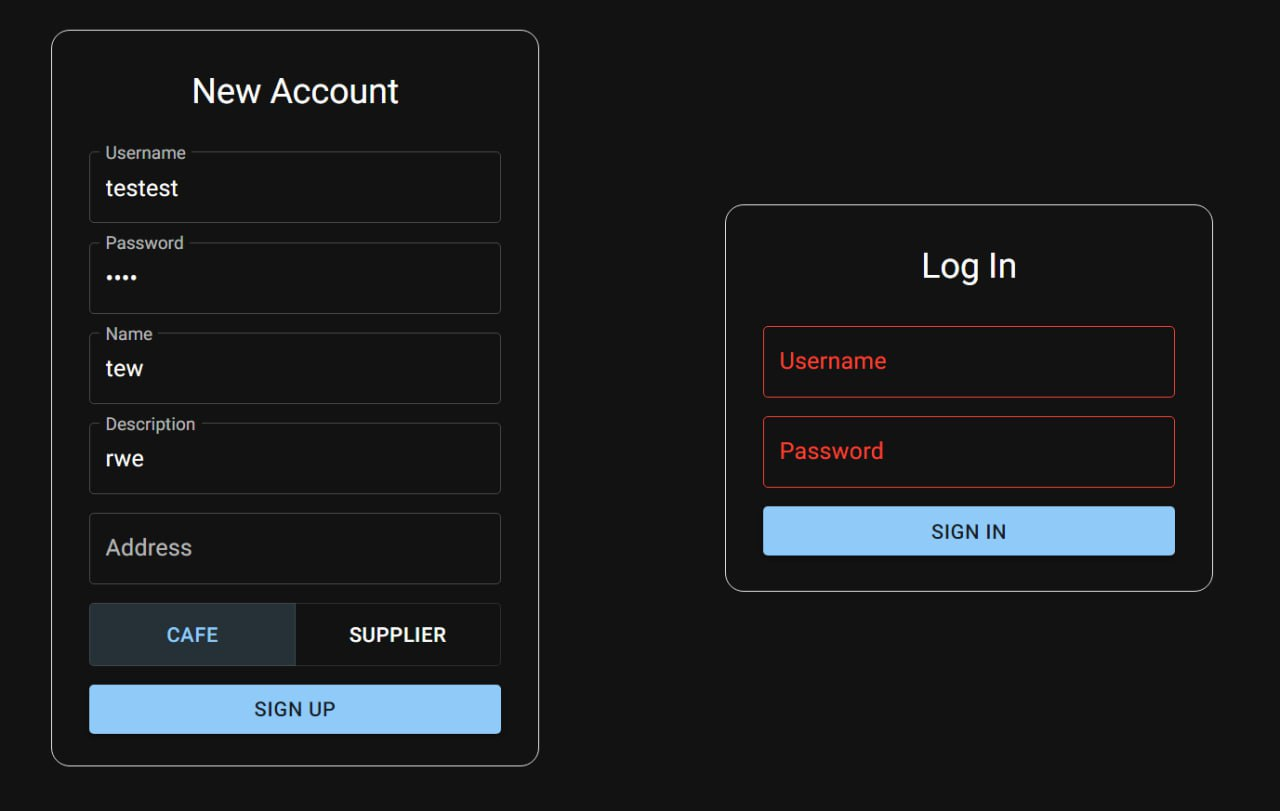
\includegraphics[width=0.7\textwidth]{fig/project-1.jpg}
  \caption{Страница аутентификации пользователей}
\end{figure}

\begin{figure}[H]
  \centering
  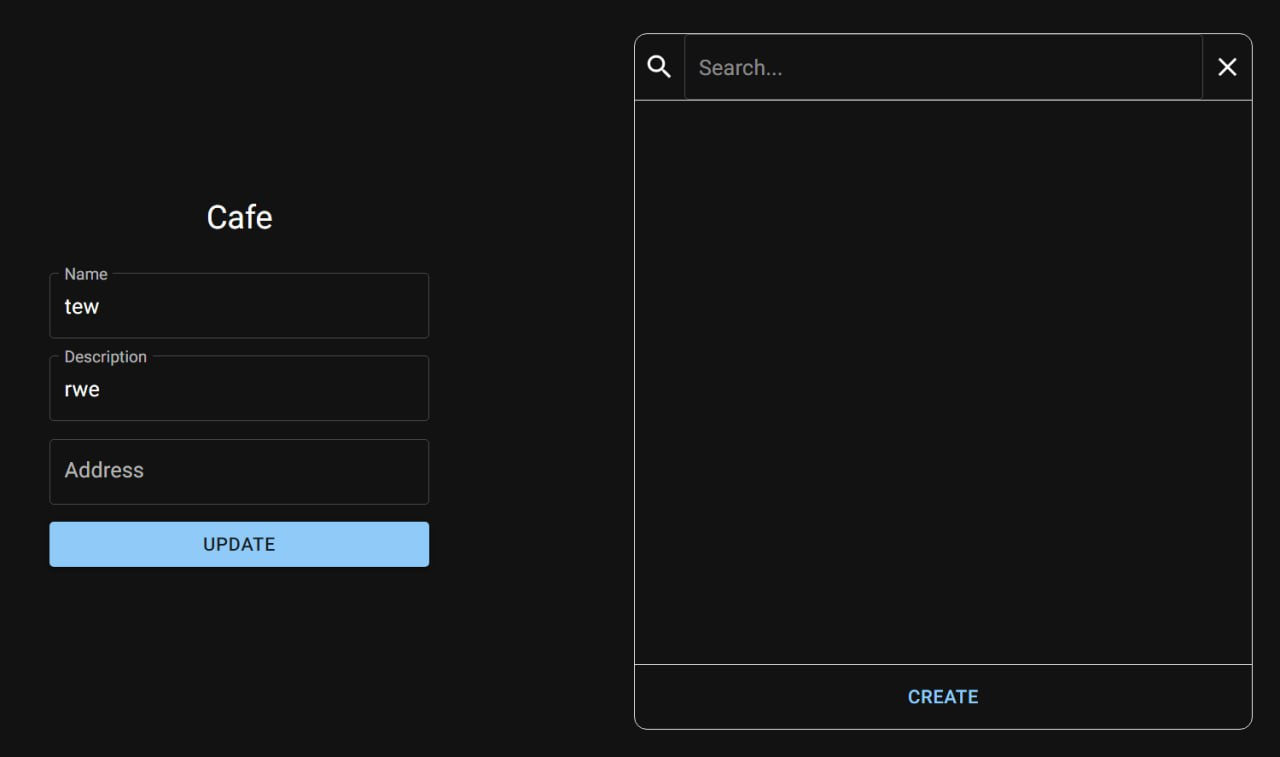
\includegraphics[width=0.7\textwidth]{fig/project-2.jpg}
  \caption{Страница владельца кафе}
\end{figure}

\begin{figure}[H]
  \centering
  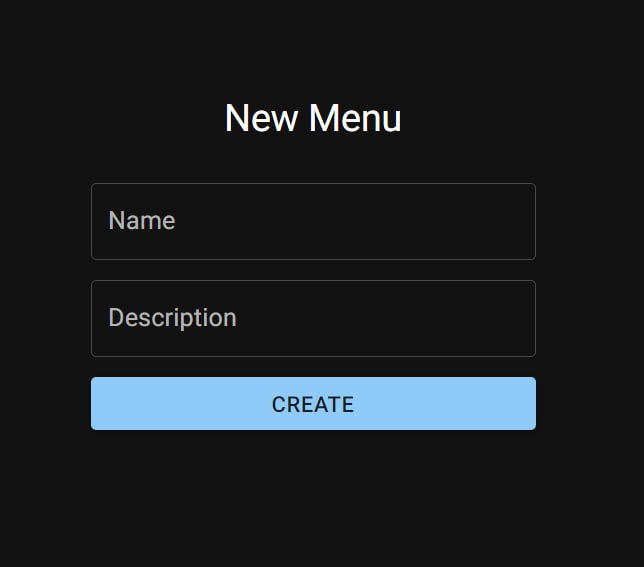
\includegraphics[width=0.5\textwidth]{fig/project-3.jpg}
  \label{}
  \caption{Создание нового меню}
\end{figure}

\begin{figure}[H]
  \centering
  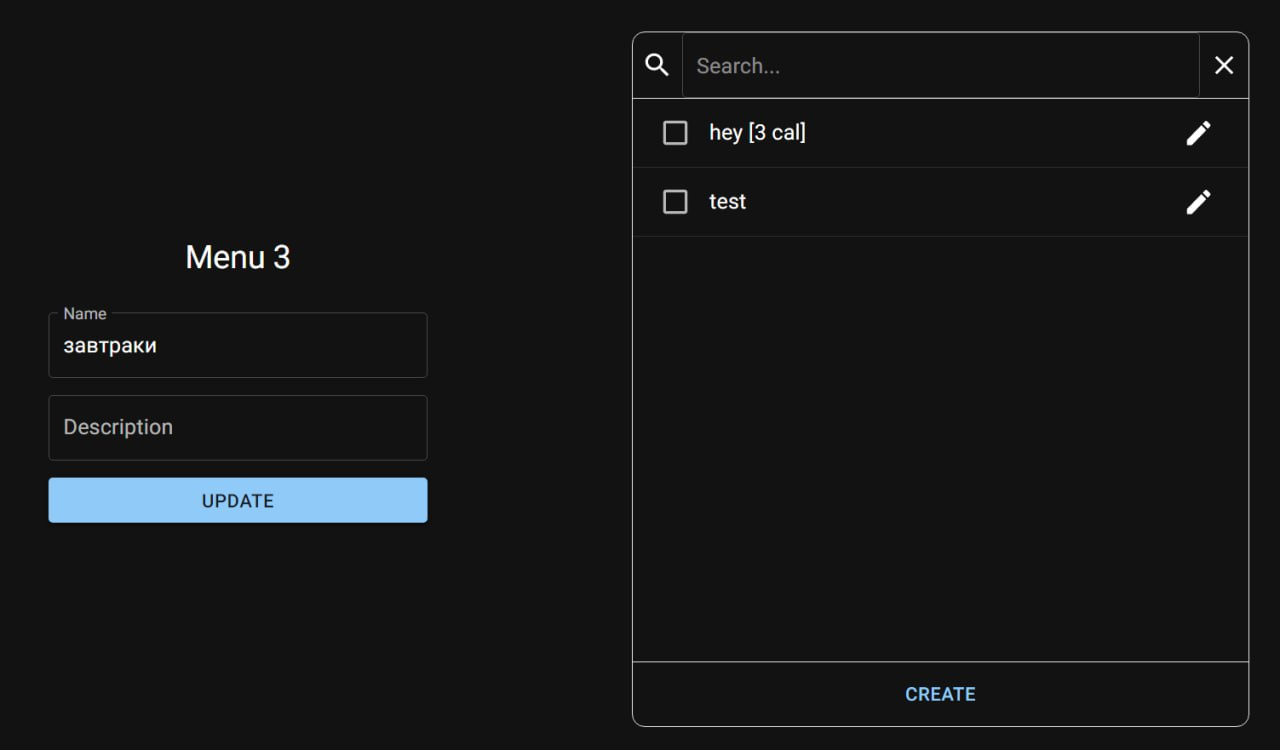
\includegraphics[width=0.7\textwidth]{fig/project-4.jpg}
  \caption{Добавление рецепта в меню}
\end{figure}

\begin{figure}[H]
  \centering
  
\includegraphics[width=0.6\textwidth]{fig/project-5.jpg}
  \caption{Поиск рецептов}
\end{figure}

\begin{figure}[H]
  \centering
  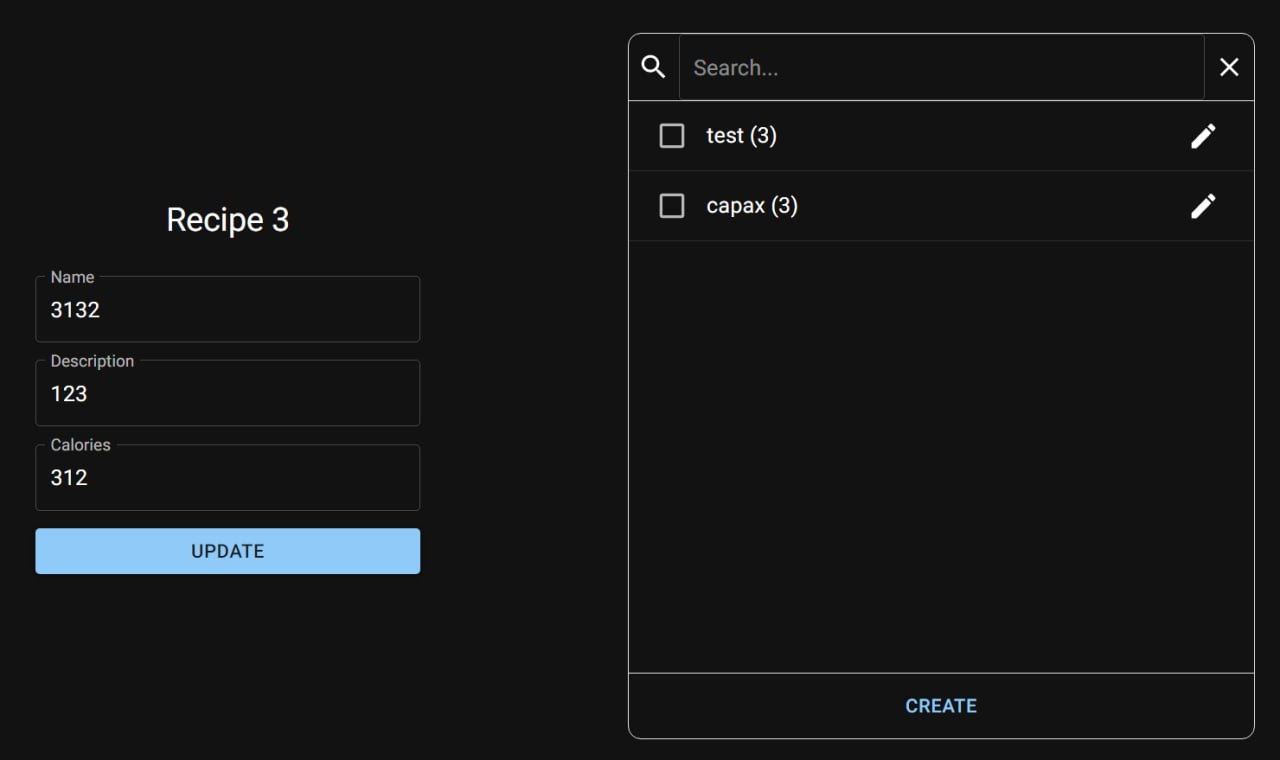
\includegraphics[width=0.7\textwidth]{fig/project-6.jpg}
  \caption{Обновление рецептов}
\end{figure}

\begin{figure}[H]
  \centering
  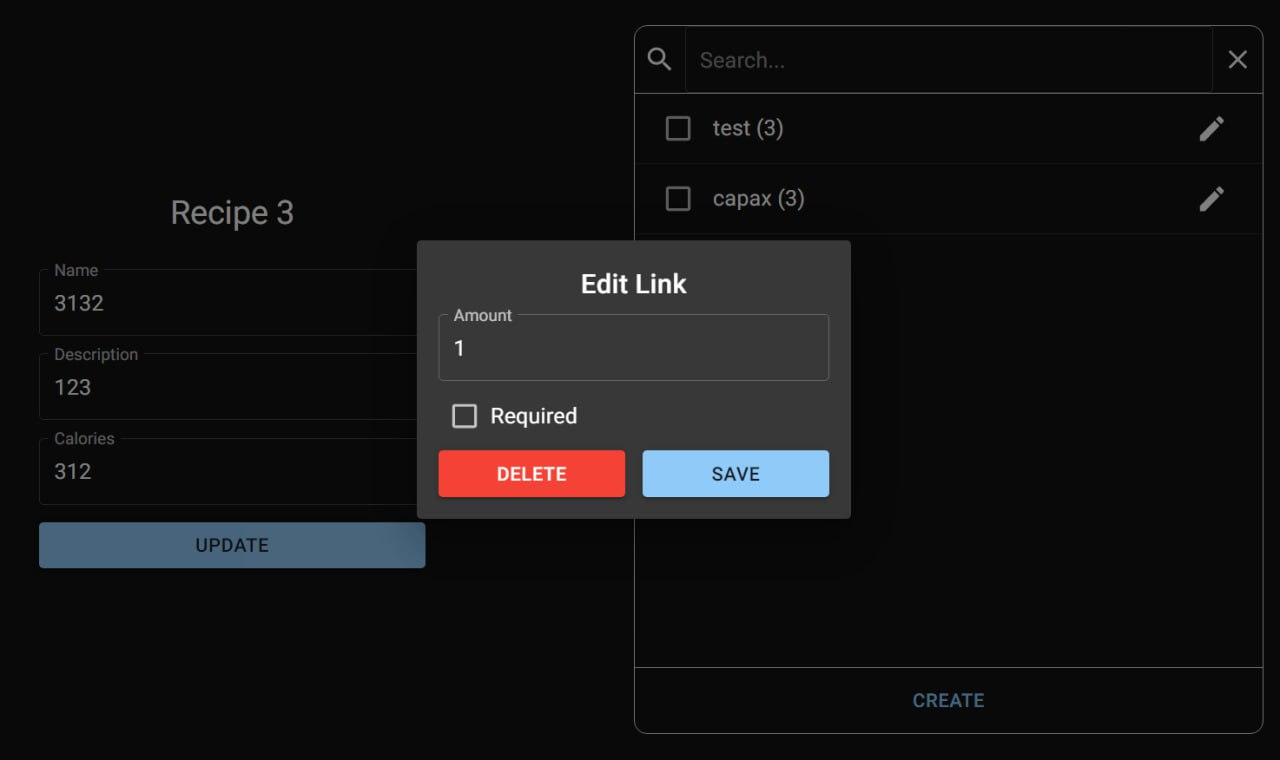
\includegraphics[width=0.7\textwidth]{fig/project-7.jpg}
  \caption{Редактирование связки ингредиент-рецепт}
\end{figure}

\begin{figure}[H]
  \centering
  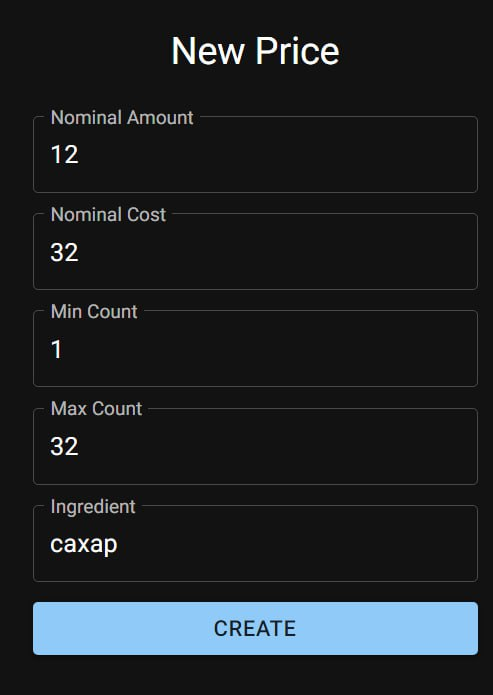
\includegraphics[width=0.4\textwidth]{fig/project-8.jpg}
  \caption{Создание лота поставщика}
\end{figure}

\begin{figure}[H]
  \centering
  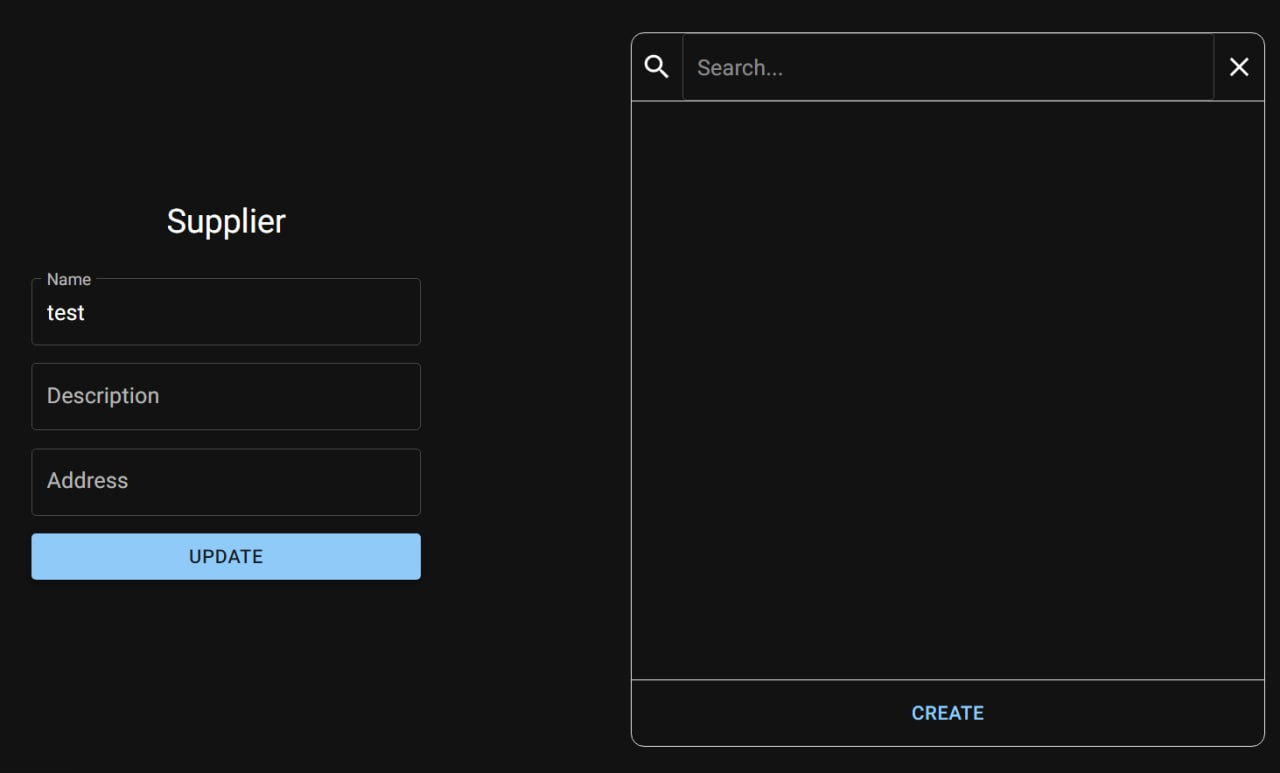
\includegraphics[width=0.7\textwidth]{fig/project-9.jpg}
  \caption{Страница поставщика}
\end{figure}



\begin{markdown}
## Ссылки
\end{markdown}

\noindent Рабочий репозиторий: \url{https://github.com/BD-term-paper/term-web-application}.

\noindent Описание на умозрение пользователей.
